\documentclass[11pt]{article}

\usepackage{float}
\usepackage{hyperref}
\usepackage{graphicx}
% formatting
\usepackage{fullpage}
\usepackage{verbatim}
\usepackage{moreverb}
\usepackage{minted}
\let\verbatiminput=\verbatimtabinput
\def\verbatimtabsize{4\relax}

\begin{document}
\title{EECS 151/251A FPGA Lab\\
Lab 1: Introduction to FPGA Development + Creating a Tone Generator}

\author{Prof. Borivoje Nikolic \\
TA: Vighnesh Iyer \\Department of Electrical Engineering and Computer Sciences\\
College of Engineering, University of California, Berkeley}
\date{}
\maketitle

\section{Before You Start This Lab}

Before you proceed with the contents of this lab, be sure that you have gone through and completed the steps involved in Lab 0. There is no checkoff for Lab 0, but there will be for this lab. Let the TA know if you are not signed up for this class on bCourses and Piazza or if you do not have a class account (eecs151-xxx), so we can get that sorted out. Also, please go through the Verilog Primer slides that are linked to on Piazza; you should feel somewhat comfortable with the basics of Verilog to complete this lab.\\

To fetch the skeleton files for this lab \verb|cd| to the git repository (\verb|labs_fa16|) that you had cloned in Lab 0 and execute the command \verb|git pull|.\\

You can find the documents/datasheets useful for this lab in the \verb|lab1/docs| folder.

\section{Our Development Platform - Xilinx ML505}
For the labs in this class, we will be using the Xilinx XUPV5-LX110T development board which is built on the ML505 evaluation platform. Our development board is a printed circuit board that contains a Virtex-5 FPGA along with a host of peripheral ICs and connections. The development board makes it easy to program the FPGA and allows us to experiment with different peripherals. The following image identifies important parts of the board:

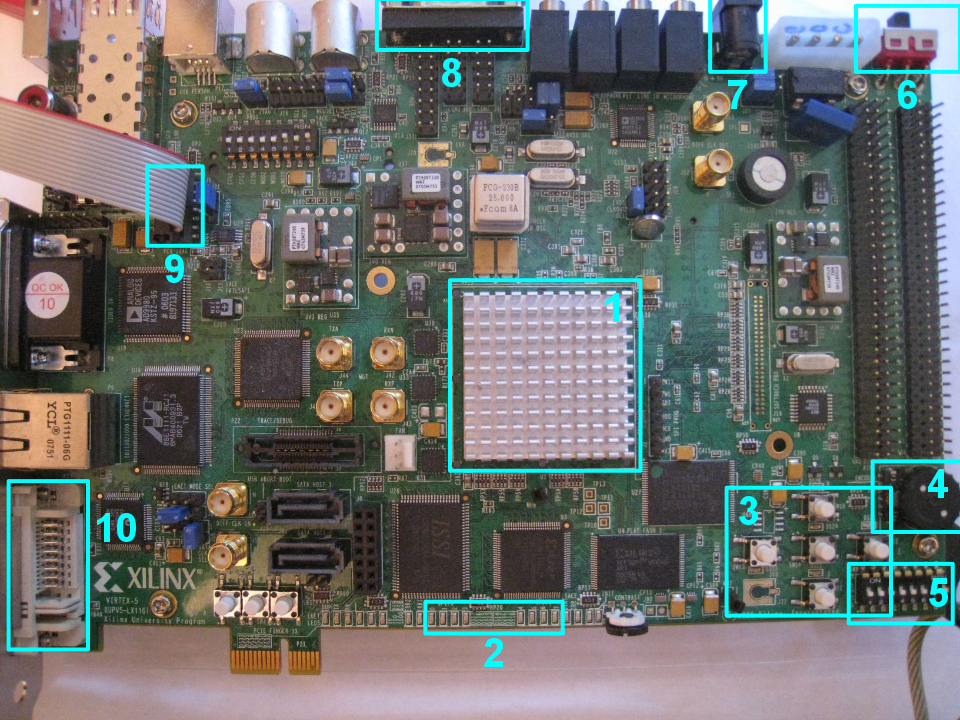
\includegraphics[width=\textwidth]{images/dev_board.png}
\begin{enumerate}
	\item Virtex-5 FPGA (covered by heat sink). It is connected to the peripheral ICs and I/O connectors via PCB traces.
	\item GPIO LEDs, numbered 0-7
	\item North, East, South, West, Center user push buttons, each with a corresponding LED
	\item Rotary encoder (a wheel we can rotate clockwise or counterclockwise and push horizontally)
	\item GPIO DIP (dual-inline package) switches, numbered 1-8 (but referred to 0-7 in code)
	\item Board power switch (toggle for a full board reset, after which you will have to reprogram the FPGA)
	\item Power connector; the power cable on many of these board is sensitive to movement and can come loose easily. Make sure you seat the power cable properly.
	\item Serial port
	\item JTAG header (used to program the FPGA, the Xilinx programmer is connected to this header)
	\item DVI-I connector (for video output)
\end{enumerate}

You will also notice a device sitting to the left of the development board that looks like this:\\

\begin{center}
	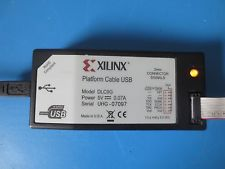
\includegraphics{images/xilinx_platform_cable.jpg}
\end{center}

This is a Xilinx FPGA programmer that connects to your workstation (desktop computer) over USB to receive a compiled bitstream file which it then sends to the development board and the FPGA over the JTAG interface. Before you run \verb|make impact| to send your design to the FPGA, make sure that the LED on the programmer is glowing green. If it is glowing yellow or not glowing at all, make sure that the wired connections are solid and that the development board is powered and on.

\section{The FPGA - Xilinx Virtex-5 LX110T}
To help you become familiar with the FPGA that you will be working with through the semester, please read Chapter 5: Configurable Logic Blocks (page 171) of the \href{http://inst.eecs.berkeley.edu/~cs150/fa11/resources/ug190.pdf}{Virtex-5 User Guide} and answer the following questions (you should be able to discuss your answers for checkoff):

\subsection{Checkoff Questions}
\begin{enumerate}
	\item How many SLICEs are in a single CLB?
	\item How many inputs do each of the LUTs on a Virtex-5 LX110T FPGA have?
	\item How many LUTs does the LX110T have?
	\item How do you implement logic functions of 7 inputs in a single SLICEL? How about 8? Draw a high-level circuit diagram to show how the implementation would look. Be specific about the elements (LUTs, muxes) that are used.
	\item What is the difference between a SLICEL and a SLICEM?
\end{enumerate}

\section{Overview of the FPGA Build Toolchain}
Before we begin the lab, we should familiarize ourselves with the CAD (computer aided design) tools that translate HDL into a working circuit on the FPGA. These tools will pass your design through several stages, each one bringing it closer to a concrete implementation.\\

Looking at the directory structure of the \verb|lab1| folder, you can see two main folders, \verb|src| and \verb|cfg|. You will also find a \verb|Makefile|. When executing parts of the toolchain, you will want to run \verb|make| in the \verb|lab1| folder. The \verb|Makefile| delegates to another \verb|Makefile| that resides in the \verb|cfg| folder. In the \verb|cfg| folder you will also find other files that are used by tools during the build process. We will discuss every step of the toolchain.\\

\subsection{Synthesis with XST}
The synthesis tool (in this case of this class, Xilinx Synthesis Tool(xst)) is the first program that processes your design. Among other tasks, it is responsible for the process of transforming the primitive gates and flip-flops that you wrote in Verilog into LUTs and other primitive FPGA elements.\\

For example, if you described a circuit composed of many gates, but ultimately of 6 inputs and 1 output, xst will map your circuit down to a single 6-LUT. Likewise, if you described a flip-flop it will be mapped to a specific type of flip-flop which actually exists on the FPGA.\\

The following figure shows the flow of files through XST. \\

\begin{center}
	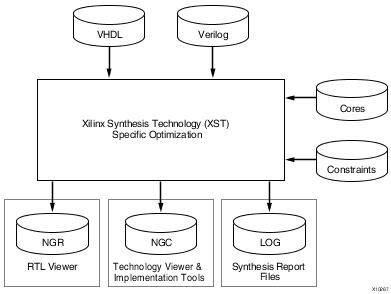
\includegraphics{images/xst_design_flow.png}
\end{center}

XST takes in Verilog and/or VHDL files to be parsed and synthesized.

XST also takes in 'Cores' which are pre-built and synthesized digital circuit blocks that provide some commonly needed functionality; they are usually provided by Xilinx to enable rapid FPGA development. They include things like pipelined dividers and multipliers, floating point units, and system buses.

XST also takes in 'Constraints' which are given in the form of a XCF file. In this lab, we don't use any constraints or cores that are passed into XST.

The outputs of XST include a LOG file, which is a text file that you can examine to make sure the synthesis succeeded, or if it failed or emitted warnings, you can see what those issues are.

Another output of XST is a NGR file which can be viewed with Xilinx ISE (as we will see soon); this file gives a high-level schematic view of how your Verilog modules are set to be implemented on the FPGA.

The final product of synthesis is a netlist file (NGC); it is a text file that contains a list of all the instances of primitive components in the translated circuit and a description of how they are connected.

\subsection{Translation and Mapping with NGDBuild and Map}
The tools that perform translation and mapping are NGDBuild and Map respectively. These tools take the output of the synthesis tool (a generic netlist) and translates each component to an equivalent on the specific Xilinx vc5vlx110t FPGAs we have in the lab. 

The translation tool merges all the input netlists and design constraint information and outputs a Xilinx Native Generic Database (NGD) file. NGDBuild takes the UCF (User Constraints File) and the NGC (from XST) files as inputs.

The mapping tool maps the logic defined by an NGD file into FPGA elements such as CLBs (configurable logic blocks) and IOBs (input/output blocks). The Map tool takes in the NGD file produced by the translation tool and produces a Xilinx Native Circuit Description (NCD) file.

\subsubsection{User Constraints File (UCF)}
We will take a small detour here to cover what a UCF is and how to add top-level signal connections to it.

A user constraints file is passed to the translation tool (NGDBuild) and it contains information regarding the top-level pin assignments and timing constraints. When you opened \verb|ml505top.v| in Lab 0, you noticed that your top-level Verilog module received several input and output signals. These signals were \verb|input [7:0] GPIO_DIP| and \verb|output [7:0] GPIO_LED|. You added some Verilog gate primitives to drive the outputs with some logic operations done to the inputs. But how do the tools know where those signals come from? That's what the UCF is for.

Open the UCF \verb|lab0/ml505top.ucf| for Lab 0 and take a look. Here you can see where the \verb|GPIO_DIP| and \verb|GPIO_LED| nets come from. Here is the syntax used to declare a top-level signal that you can sense and/or drive from your top-level Verilog module.

\begin{minted}{verilog}
	NET (net name)<bit index> LOC="(FPGA pin number)"
	NET (net name)<bit index> IOSTANDARD="(voltage level)"
\end{minted}

The (net name) is the signal name that is presented to your top-level Verilog module. The bit index can be set optionally for a multi-bit signal for the same net name. The LOC defines what pin coming out of the FPGA contains that signal. All the pins coming out of the FPGA's BGA package are labeled, and this is how we can tap or drive signals from a particular pin. The second line defines an IOSTANDARD for a given net; this is just a statement of the voltage level for a given pin. Here is an example for a \verb|GPIO_LED|

\begin{minted}{verilog}
NET GPIO_LED<0> LOC="H18";
NET GPIO_LED<0> IOSTANDARD="LVCMOS25";
\end{minted}

These 2 lines give you access to a net called \verb|GPIO_LED| in your top-level Verilog module. This net is connected to the \verb|H18| pin coming out of the FPGA which is routed on the PCB to LED0 on the board via a trace.

Note that this declaration doesn't specify whether the net is an input or output; that is defined in your Verilog top-level module port declaration.

On the ML505 development board, we can utilize what is called a master UCF file to make adding signals to your design easy. This master UCF file is used in conjunction 



\subsection{Place and Route with PAR}
Now we resume where we left off after the mapping tool. The map tool's NCD output file is fed into the Place and Route tool which is called PAR. PAR places and routes the design that was generated by Map, and it outputs another NCD file with placement and routing information. This process is often the most time consuming of any of the steps in the toolchain; the algorithms used for placement and routing are quite sophisticated and have long run times.

\subsection{Bitstream Generation with BitGen}
The fully placed and routed design from PAR as a NCD file is now ready to be translated into another file that the Xilinx FPGA programmer can understand. We use a tool called BitGen to perform the generation of the bitstream that is sent to the FPGA. This is the last step in the FPGA build process, and it produces a .bit file which can be uploaded to the FPGA via the programmer.

\subsection{Timing Analysis with TRCE}
The \verb|Makefile| we use in this class performs an additional step after running BitGen. To verify that our design met all timing requirements and to see a timing analysis, we use a tool called Trace (TRCE) which takes in output files generated by PAR and produces a timing report. It will let you know what is the maximum clock speed your design can operate at reliably.

\subsection{Report Generation with ISE}
A very important precaution to take after running each step of the toolchain is to verify that there are no errors or warnings that a given tool produced. We use a program called xreport which ships with Xilinx ISE to produce a report detailing the status of each build tool. To run this tool, execute \verb|make report| in the \verb|/lab1| directory. The tool will give you all the warnings and errors emitted by each tool in a GUI. It will also report the resource usage of your design.

\subsection{FPGA Programming with iMPACT}
Finally, to send the bitstream file you generated with BitGen to the FPGA, we use a tool called iMPACT. To execute this tool run \verb|make impact| in the \verb|/lab1| directory after the regular \verb|make| process has completed and succeeded without any errors. After this tool runs, your design will be configured and active on the FPGA.

\subsection{Toolchain Conclusion}
All of this information is dense and complex. Don't worry about understanding the internals of each tool and the exact file formats they work with. Just understand what each step of the toolchain does at a high level and you will be good for this class. We use all these tools regularly, but executing them is all handled by the staff provided \verb|Makefile|.

\section{A Structural and Behavioral Adder Design + Using fpga\_editor and the FPGA schematic}

\subsection{Structural 2-bit Adder}
Navigate to the \verb|/lab1/src| directory.

\subsubsection{Inspection Using Schematic and fpga\_editor}

\subsection{Behavioral 4-bit Adder}

\subsubsection{Inspection Using Schematic and fpga\_editor}

\section{Designing a Tone Generator}

\subsection{Piezoelectronic Buzzers}

\subsection{Finding the Piezo in the Schematic}

\subsection{Adding the Piezo signal to the UCF File}

\subsection{Generating a square wave}

\subsection{Switching the Wave On and Off}

\section{Simulating Your Tone Generator}

% This will be a gentle intro to what is done in the next lab
\section{Optional: Use Remaining Switches to Control Frequency or Duty Cycle}

% Reserve for the next lab, this can be tough since it involves synchronization and edge triggered sampling of phase differences
%\section{Using the Rotary Encoder to Switch Frequencies}

\end{document}
